\section{Definições}\label{sec:defs}

\begin{defi}[Corpo Rígido]
  Um corpo rígido $cr$ é definido por dois subconjuntos disjuntos de parâmetros
  $cr= \langle \hat{cr}, \bar{cr} \rangle$ em que:

  \begin{itemize}
    \item $\hat{cr} = \langle pos, \theta, vel, \omega \rangle$, que são os
      parâmetros de estado mutáveis, respectivamente: posição ($\mathbb{R}
      ^{3}$), orientação ($\mathbb{R} ^{3}$), velocidade linear ($\mathbb{R}
      ^{3}$), velocidade angular ($\mathbb{R} ^{3}$)

    \item $\bar{cr} :$ parâmetros imutáveis do corpo que descrevem sua natureza
      fixa e que permanecem constantes ao longo do curso de planejamento.
  \end{itemize}
\end{defi}

Exemplos de parâmetros considerados nesta modelagem imutáveis são: coeficiente
de atrito estático e dinâmico, descrição $3D$ do corpo (por exemplo, por meio de
um conjunto de primitivas $3D$), centro de massa no referencial do corpo,
coeficiente de restituição, coeficiente de amortecimento linear e angular.

\begin{defi}[Bola]\label{def:bola}
  Bola é um corpo rígido $b$, no qual somente as componentes $\langle x,y
  \rangle$ do parâmetro $\hat{b}.pos$ são observáveis.
\end{defi}

De acordo com a arquitetura do jogo descrita na Seção~\ref{sec:arch_ssl}, tem-se
que, a partir de uma sequência de quadros, é possível obter um valor estimado
para o parâmetro $\hat{b}.vel$ a partir do intervalo entre os dados recebidos da
\textit{SSL-Vision} e da equação $ vel \approxeq \frac{\Delta pos}{\Delta t} $.
Entretanto, uma vez que a componente $z$ de $\hat{b}.pos$ não é observável,
$\hat{b}.vel.z$ não pode ser estimada a partir do intervalo entre os dados
recebidos da \textit{SSL-Vision}. Semelhantemente,  uma vez que o parâmetro
$\hat{b}.\theta$ também não pode ser observado, não se pode estimar o valor de
$\hat{b}.\omega$ com exatidão.

% XXX[vbramigk] definir skill

\begin{defi}[Robô]
  Robô, representado por $r$, é um conjunto de sistemas compostos de corpos
  rígidos, \textit{hardware} e \textit{firmware}. Neste trabalho será
  considerado que o robô tem os seguintes sistemas:

  \begin{itemize}
    \item Drible: imprime um torque a bola;
    \item Chute baixo: imprime uma força à bola $b$ e, possivelmente, um torque,
      com o objetivo de alterar as componentes $\langle x,y \rangle$ do
      parâmetro $\hat{b}.vel$;
    \item Chute alto: imprime uma força à bola $b$ e, possivelmente, um torque,
      com o objetivo de alterar as componentes $\langle x,y,z \rangle$ do
      parâmetro $\hat{b}.vel$, com $\hat{b}.vel_z \neq 0$;
    \item Receptor: recebe comandos enviados pelo sistema de transmissão de seu
      respectivo time;
    \item Sistema de movimentação: imprime uma força e um torque ao centro de
      massa global do $r$.
  \end{itemize}
\end{defi}

A Figura~\ref{fig:rob_data} ilustra os parâmetros de estado mutáveis do robô.
Por meio dos sistemas listados acima, cada robô $r$ pode executar um conjunto de
ações $A_{rob}$. A Figura~\ref{fig:robo} apresenta os atuadores típicos de um
robô da SSL.

\begin{figure}[H]
  \centering
  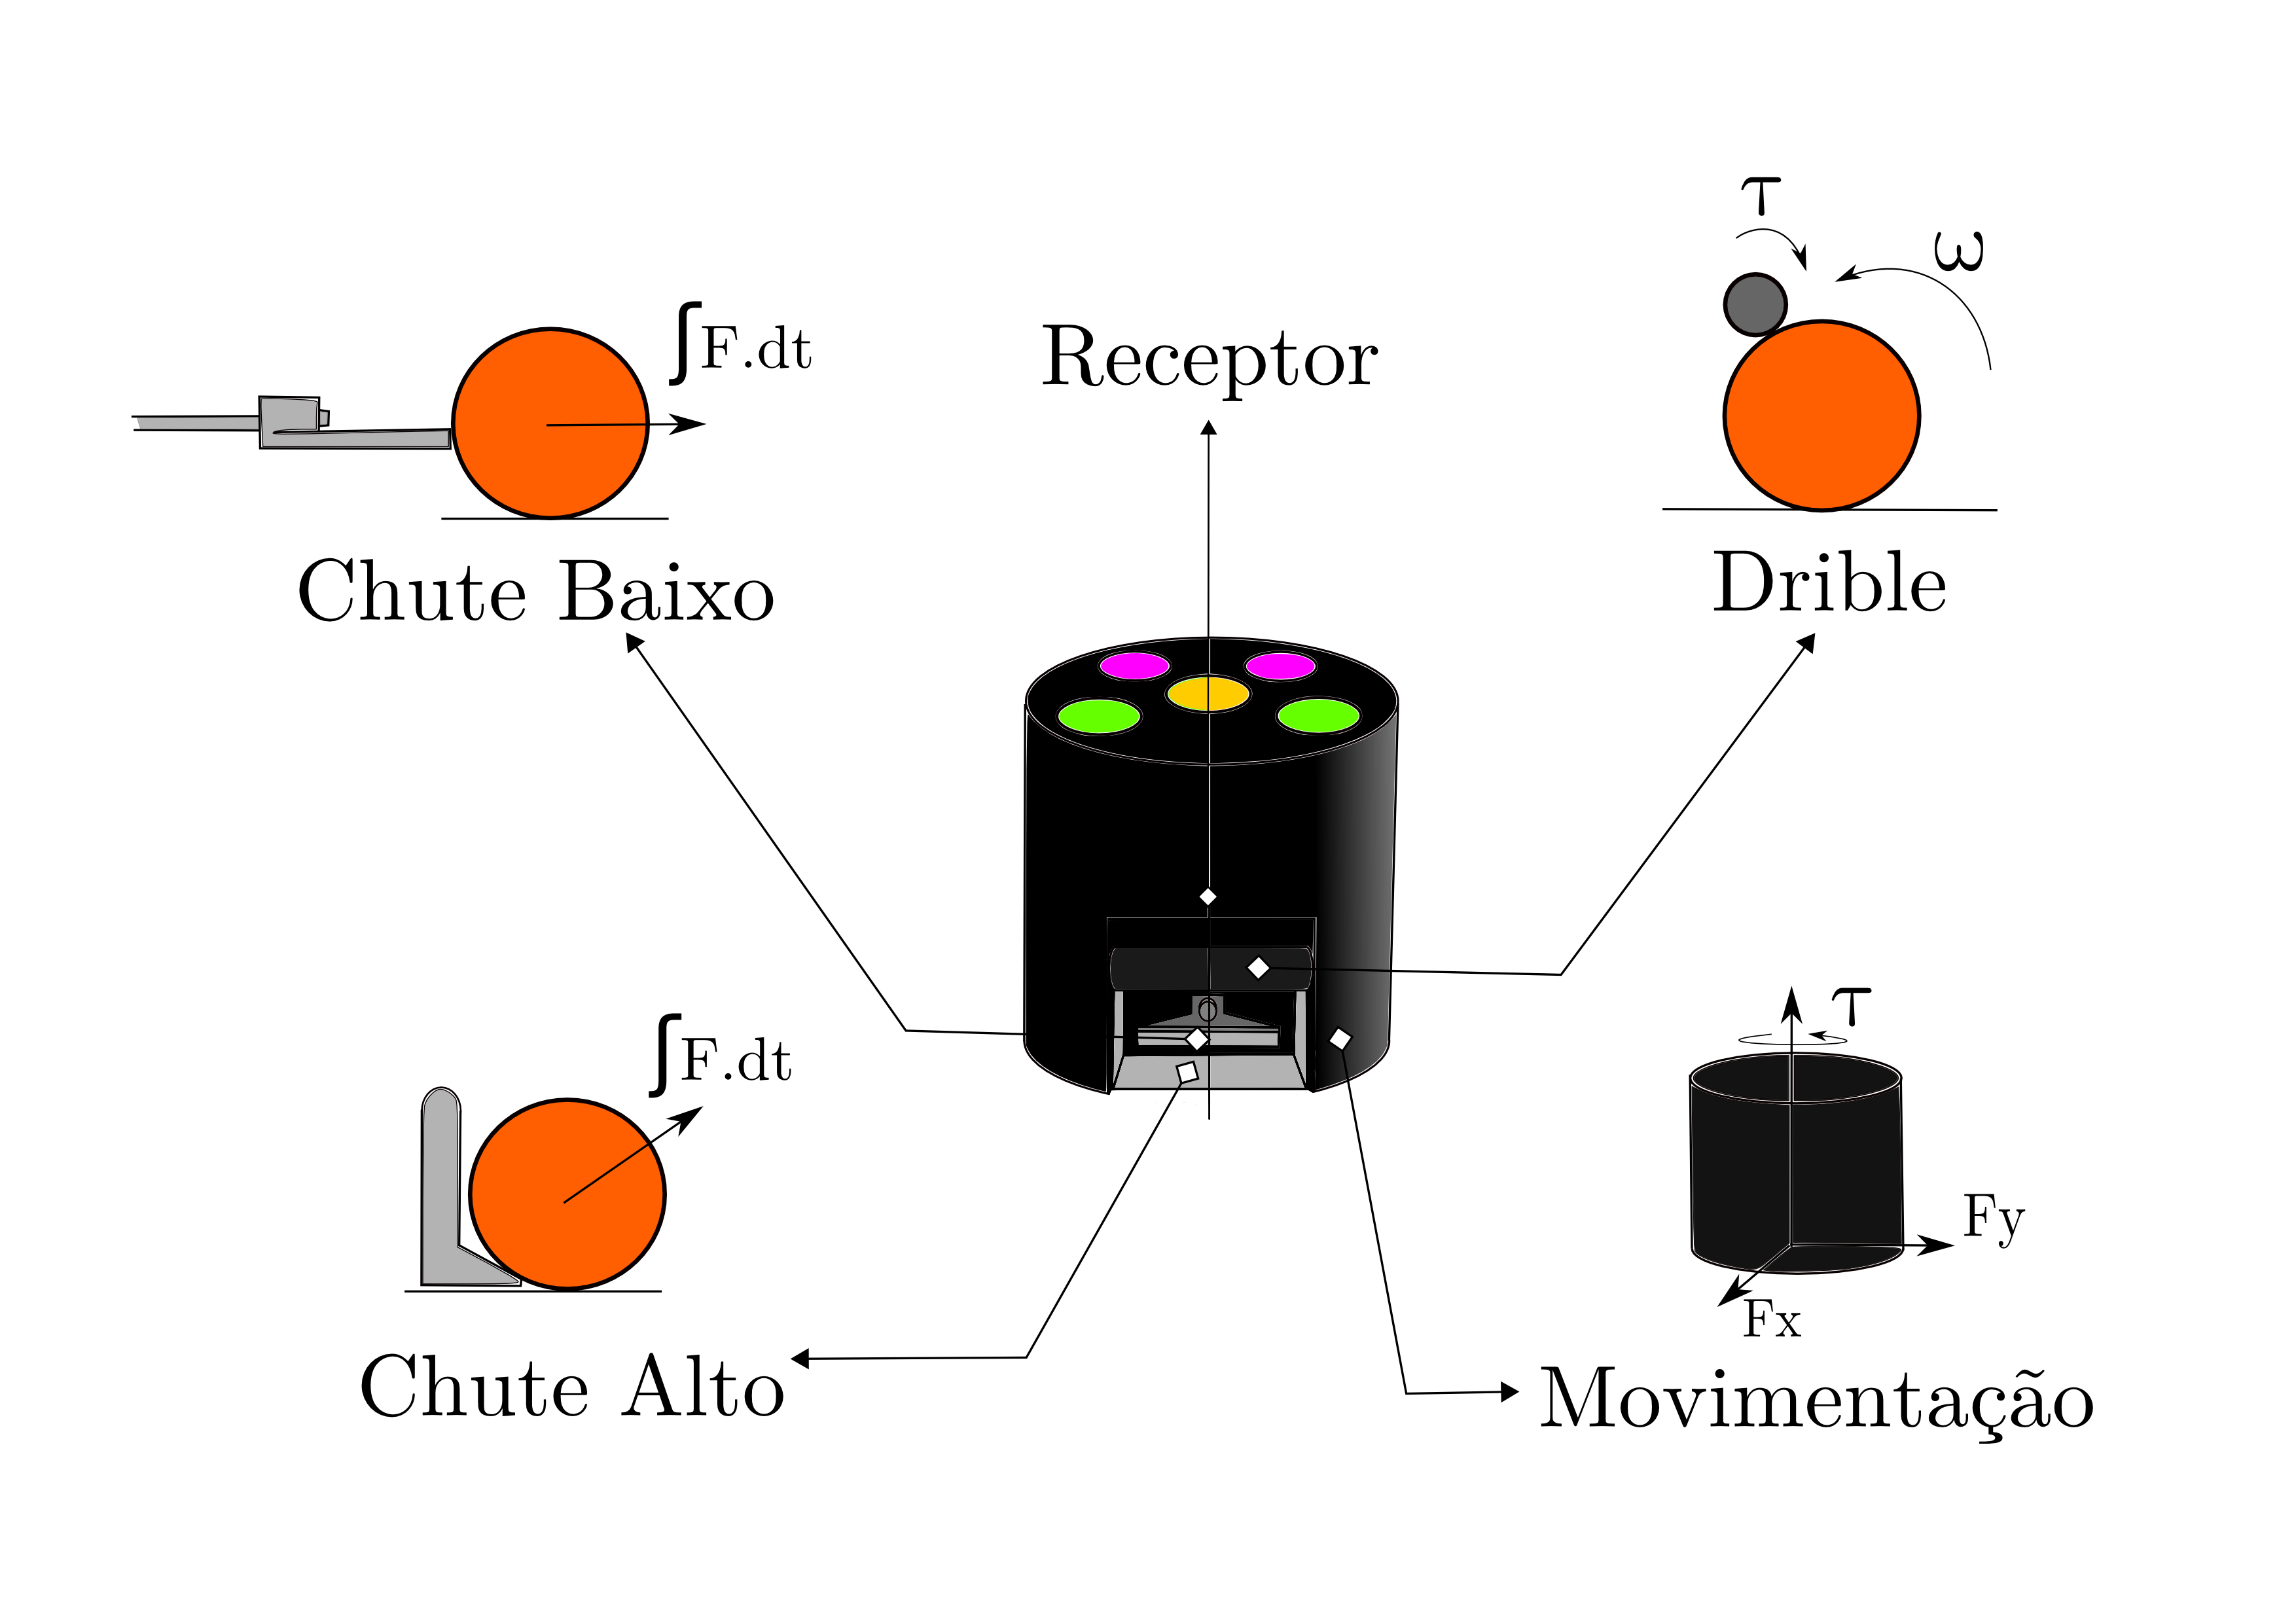
\includegraphics[width=0.8\linewidth]{robo}
  \caption{Atuadores típicos de um robô da SSL}\label{fig:robo}
\end{figure}

Apesar de o modelo descrito acima abranger a maioria dos robôs utilizados
atualmente por equipes da SSL, é importante ressaltar que o robô pode ter um
conjunto de sensores que poderiam coletar informações adicionais às transmitidas
pela \textit{SSL-Vision} juntamente com um sistema de transmissão para enviá-las
ao software do seu respectivo time. Isso é interessante, pois, conforme
observado na Definição~\ref{def:bola}, o parâmetro $\hat{b}.\theta$ não é
observável. Como o sistema de drible impõe um torque à bola, por meio de um
sensor, é possível estimar o valor de $\hat{b}.\omega$. Sem esse sensor, não é
possível prever com exatidão a trajetória da bola somente com informações de
simulação ou da visão.


% TODO: referenciar zicler para exemplos de skills
% TODO: Discrever Skill
%\begin{defi}[Skill]
%  $Sk \subset A_{rob}$ um conjunto de \textit{skills};
%\end{defi}
%
%% TODO: Discrever Tactic
%\begin{defi}[Tactic]
%  $tk = G(V \in Sk, E \in {prob} )$ o conjunto de todas as táticas possíveis
%  formadas a partir de grafos orientados, em que os vértices são \textit{skills} $sk \in Sk$
%  e as arestas são $prob$ associadas a possibilidade de ocorrerem as transições
%  entre uma skill e outra;
%
%% XXX: wtf???
%  $prob: X \longrightarrow [0,1]$ uma distribuição de probabilidade, cujo argumento é
%  $x \in X$;
%\end{defi}
%
%% TODO: Definir agente baseado em utilidade
%\begin{defi}[Tactic]
%  $f_{U}: X \longrightarrow \mathbb{R^{+}} \cup\lbrace 0\rbrace$ uma função utilidade tal que
%  $f_{U}(x)$ reflate a utilidade do estado $x \in X$ um entre estados do mundo dado os estados;
%\end{defi}
%
%% TODO: Definir árvore de busca
%\begin{defi}[Árvore de Busca]
%  $AB =\lbrace V \subset X, E \subset A\rbrace$ uma árvore de busca;
%\end{defi}
%
%% TODO: Definir estratégia (pode ser o BK-BGK)
%\begin{defi}[Estratégia de Busca]
%  $e_b: \langle X_{ob}^{i}, e, f_{U}, r_i, AB\rangle \longrightarrow AB^{'}$ uma estratégia de busca.
%\end{defi}
%
%% TODO: Modelo de reação dos robôs do time adversário
%\begin{defi}[Modelo de reação dos robôs do time]
%  Depende de quão distante no tempo está a reação que se quer
%  estimar. Quanto menor a distância no tempo, mais este modelo
%  se aproxima do modelo dinâmico dos robôs.
%\end{defi}

\begin{defi}[Time]\label{def:time}
  Sejam os seguintes parâmetros:

  \begin{description}
    \item $Rob_c$ o conjunto dos robôs controlados;
    \item $Rob_{ad}$ o conjunto dos robôs adversários, isto é, não controlados;
    \item $X$ o espaço de estado de todos os corpos rígidos envolvidos na partida considerada;
    \item $x_{init} \in X$ o estado inicial;
    \item $X_{goal}\subset X$ o conjunto de estados objetivo;
    \item $x_{ob}^{i}$ os estados observados pelo módulo \textit{SSL-Vision} no instante $i$;
    \item $X_{ob}^{i} =  \lbrace{x_{ob}^{0} = x_{init},\dots,x_{ob}^{i}}\rbrace$;
    \item $Sk \subset A_{rob}$ um conjunto de \textit{skills};
    \item $prob: X \longrightarrow [0,1]$ uma distribuição de probabilidade, cujo argumento é
      $x \in X$;
    \item $tk = G(V \in Sk, E \in {prob} )$ o conjunto de todas as táticas possíveis
      formadas a partir de grafos orientados, em que os vértices são \textit{skills} $sk \in Sk$
      e as arestas são $prob$ associadas a possibilidade de ocorrerem as transições
      entre uma skill e outra;
    \item $A_c = A_{rob 1} \cup \dots \cup A_{rob n_c}$ o conjunto das ações possíveis de $Rob_c$;
    \item $A_{ad} = A_{rob 1} \cup \dots \cup A_{rob n_{ad}}$ o conjunto das ações possíveis de $Rob_{ad}$;
    \item $A = A_c \cup A_{ad}$ o conjunto das ações possíveis de $Rob_c \cup Rob_{ad}$;
    \item $e: \langle x,a \rangle \longrightarrow x^{'}$ a função de transição de estado que pode
      aplicar uma ação $a\in A$ em um estado particular
      $x \in X$ e computar o estado seguinte $x^{'} \in X$;
    \item $f_{U}: X \longrightarrow \mathbb{R^{+}} \cup\lbrace 0\rbrace$ uma função utilidade tal que
      $f_{U}(x)$ mede a utilidade do estado $x \in X$ um entre estados do mundo dado os estados;
    \item $m_{reac{\ }ad}: \langle A_{ad}, X_{ob}^{i}\rangle \longrightarrow a_{ad}^{'}$ o modelo de reação dos robôs
      adversários dado $X_{ob}^{i}$;
    \item $AB =\lbrace V \subset X, E \subset A\rbrace$ uma árvore de busca;
    \item $e_b: \langle X_{ob}^{i}, e, f_{U}, m_{reac{\ }ad}, AB\rangle \longrightarrow AB^{'}$ uma estratégia de busca.
  \end{description}

  Então, um time $T$ é definido por:
  \[
    T: \langle Rob_c, A, X_{ob}^{i}, e, e_b, m_{reac{\ }ad} \rangle \longrightarrow a_c^{i+1}
  \]
\end{defi}

Assim, utilizando-se de $e$, $T$ pode simular várias sequência de ações $a_c$
dado $X_{ob}^{i}$ a partir de $f_{U}$ e $e_b$. Pode-se, a partir de $m_{reac{\
}ad}$, considerar as ações do time adversário baseado em estados anteriores.

% TODO: describe more the notation
\begin{defi}[Partida]
  Dado dois times $T_1$ e $T_2$. Uma partida $p$ é definida por:

  \[
    p = \lbrace T_1, T_2, \Delta t, \delta t, \langle Ref^{0}, X_{ob}^{0}, A_1^{0}, A_2^{0}\rangle, 
    \dots, \langle Ref^{N}, X_{ob}^{N}, A_1^{N}, A_2^{N} \rangle \rbrace
  \]

  Uma sequência, em que:
  \begin{description}
    \item $\Delta t$ é o tempo de duração da partida;
    \item $\delta t$ é o tempo médio entre cada frame enviado pela \textit{SSL-Vision} ao longo de $\Delta t$;
    \item $N \approxeq \frac{\Delta t}{\delta t}$ é número total de frames enviados pela \textit{SSL-Vision}
      ao longo de $\Delta t$;
    \item $Ref^{i}$ são os comandos enviados pelo módulo \textit{Referee-Box} no instante $i$;
    \item $X_{ob}^{i}$ são os dados enviados pelo módulo \textit{SSL-Vision} no instante $i$;
    \item $A_1^{i}$ são as ações executadas por $T_1$ no instante $i$;
    \item $A_2^{i}$ são as ações executadas por $T_2$ no instante $i$.
  \end{description}
\end{defi}

Conforme citado em na Seção~\ref{sec:arch_ssl}, $\delta t$ normalmente é $16,6{\ }ms$.
Um exemplo de $A^{i}$ pode ser visto na Figura~\ref{fig:default_atq}.

\begin{defi}[Logs]
  Dada uma partida $p$. O $log$ de $p$ é definidor por:

  \[
    log(p) = \lbrace p.\langle Ref^{0}, X_{ob}^{0}\rangle, \dots, p.\langle Ref^{N}, X_{ob}^{N}\rangle \rbrace
  \]
\end{defi}

A principal diferença entre uma partida $p$ e $log$ é o desconhecimento das
ações que levaram aos movimentos observados nas partidas. Isso é um metadado
importante quando se quer utilizar os dados de um jogo para aproximar o
comportamento de algum time (i.e., $m_{reac{\ }ad}$).  Este é um problema que
está fora do escopo deste trabalho. Um exemplo de uma abordagem para esse
problema pode ser encontrado em \cite{vail2008crf}.

% vim: tw=80 et ts=2 sw=2 sts=2 ft=tex spelllang=pt_br,en
